% ------------------------------------------------
\StartChapter{Methodology: GemGNN Framework}{chapter:methodology}
% ------------------------------------------------

\section{Notation}

\begin{table}[h!]
\centering
\begin{tabular}{ll}
\toprule
\textbf{Notation} & \textbf{Description} \\
\midrule

% --- Group 1: Problem Formulation & Data ---
\multicolumn{2}{l}{\emph{Problem Formulation \& Data}} \\
$\mathcal{L}, \mathcal{U}, \mathcal{T}$ & Sets of labeled, unlabeled, and test news articles. \\
$K$ & Number of labeled examples per class (K-shot setting). \\
$y_i, \hat{y}_i$ & Ground-truth and predicted label for a news article. \\

% --- Group 2: Heterogeneous Graph Structure ---
\multicolumn{2}{l}{\emph{Heterogeneous Graph Structure}} \\
$G=(V, E)$ & A heterogeneous graph with nodes $V$ and edges $E$. \\
$V_n, V_i$ & The sets of news nodes and synthetic interaction nodes. \\
$\mathbf{x}_v, \mathbf{h}_v$ & Initial features and learned representation for a node $v$. \\

% --- Group 3: Key GemGNN Contributions ---
% Highlighting the symbols that represent the core innovations.
\multicolumn{2}{l}{\emph{Key GemGNN Contributions}} \\
$I_i$ & Set of \textbf{synthetic user interactions} for a news article $n_i$. \\
$k$ & Number of neighbors for \textbf{Test-Isolated KNN} construction. \\
$\mathcal{V}$ & Number of views in the \textbf{Multi-View architecture}. \\
$\mathbf{h}_v^{(\nu)}$ & Representation of node $v$ in the $\nu$-th view. \\

\bottomrule
\end{tabular}
\end{table}

\section{Framework Overview}

The GemGNN (Generative Multi-view Interaction Graph Neural Networks) framework addresses the fundamental challenges of few-shot fake news detection through a novel heterogeneous graph-based approach that eliminates dependency on user propagation data while maintaining the benefits of social context modeling. Our architecture represents a systematic solution to three critical limitations in existing approaches: (1) the unavailability of real user interaction data due to privacy constraints, (2) the poor performance of existing methods in few-shot scenarios, and (3) the lack of rigorous evaluation protocols that prevent information leakage between training and test sets.

\begin{figure}[h]
    \centering
    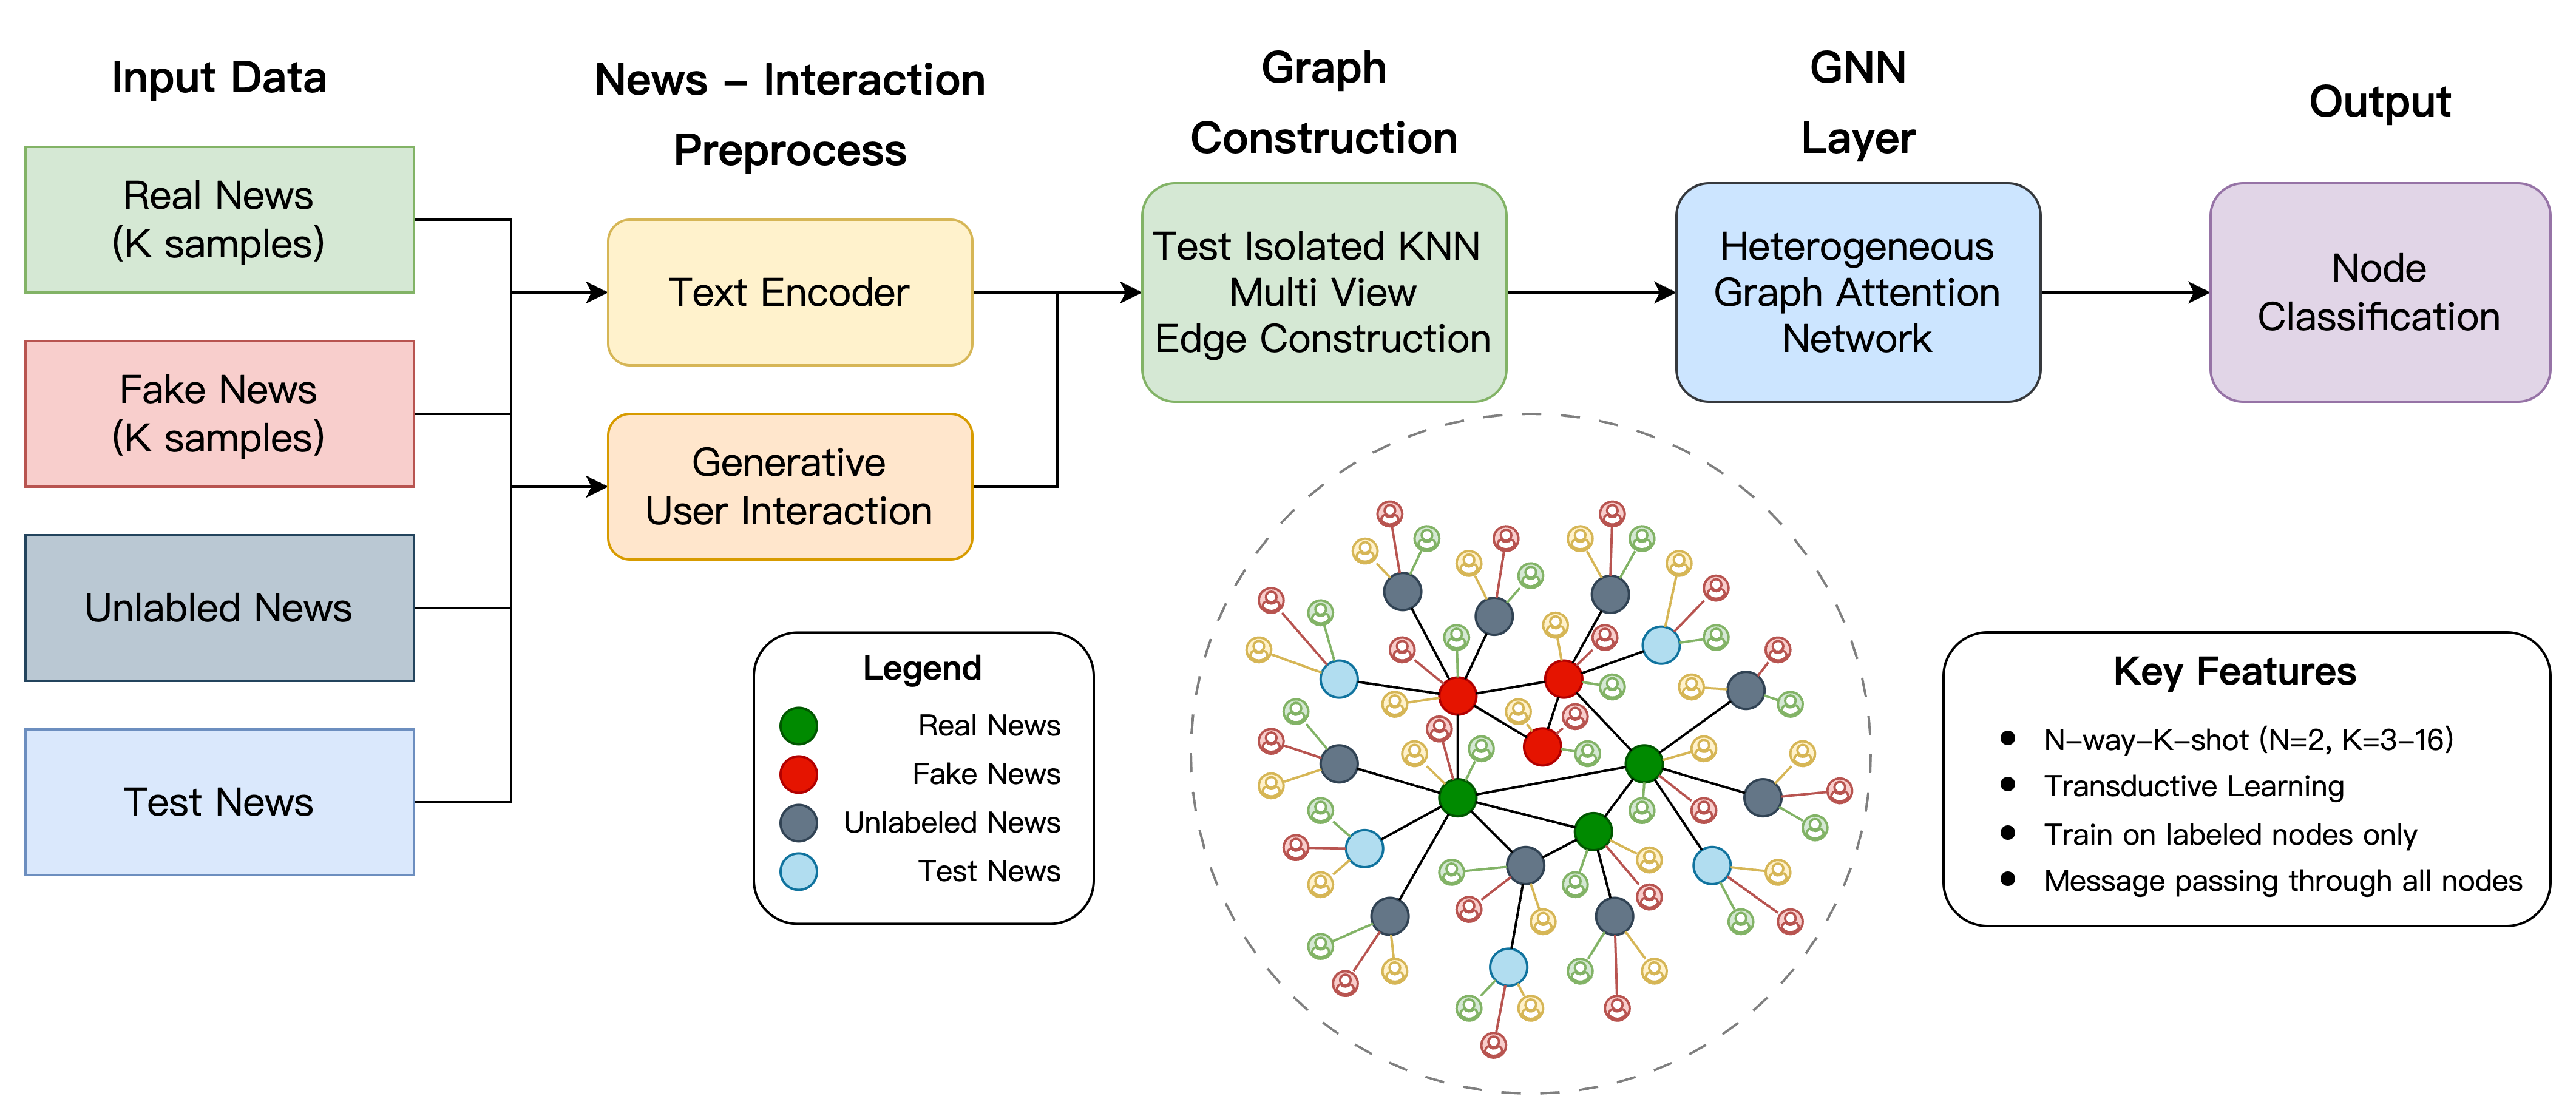
\includegraphics[width=0.8\textwidth]{context/methodology/fig/pipeline.png}
    \caption{Complete GemGNN pipeline showing data flow from news articles through heterogeneous graph construction to final classification}
    \label{fig:pipeline}
\end{figure}

The complete architecture consists of four interconnected components that work synergistically to achieve robust few-shot performance (see Figure~\ref{fig:pipeline}): (1) \emph{Generative User Interaction Simulation} using Google's Gemini LLM to create realistic social context without privacy concerns, (2) \emph{Adaptive Graph Construction} with configurable edge policies (traditional KNN vs test-isolated KNN) to balance performance optimization with evaluation realism, (3) \emph{Multi-View Graph Architecture} that leverages DeBERTa's disentangled attention structure to capture complementary semantic perspectives, and (4) \emph{Heterogeneous Graph Neural Network} with enhanced training strategies specifically designed for few-shot learning scenarios.

\textbf{Core Design Philosophy:} Our approach operates under a transductive learning paradigm where all nodes (labeled, unlabeled, and test) participate in heterogeneous message passing, but only labeled nodes contribute to loss computation. This design philosophy maximizes the utility of limited supervision by leveraging the heterogeneous graph structure to propagate information from labeled news nodes to unlabeled and test nodes through learned type-specific attention mechanisms. The framework maintains strict separation between training and test data when required, while allowing flexible adaptation to different deployment scenarios through configurable graph construction policies.

\textbf{Implementation Architecture:} The framework is implemented through two primary components that reflect our systematic approach to heterogeneous graph construction and training. The graph construction pipeline handles the complete process from news article processing through heterogeneous graph creation, while the training pipeline provides specialized few-shot learning strategies with enhanced loss functions and early stopping criteria.

Our approach begins with pre-trained DeBERTa embeddings~\cite{he2021deberta} for news articles, which provide rich semantic representations (768-dimensional vectors) that capture contextual relationships and linguistic patterns indicative of misinformation. These embeddings serve as the foundation for both similarity-based graph construction and node feature initialization in our heterogeneous graph neural network, ensuring that the model can leverage state-of-the-art natural language understanding capabilities within the graph-based architecture.

\section{Dataset Sampling Strategy}

A critical aspect of our methodology is the systematic approach to sampling training data that ensures balanced and effective few-shot learning. Our sampling strategy maximizes the utility of limited labeled data while providing sufficient unlabeled context for effective transductive learning.

\subsection{Labeled Node Sampling}

For k-shot learning scenarios, we sample exactly k labeled examples per class from the training set, following established few-shot learning protocols~\cite{wang2020fewshot, finn2017model}. The sampling process ensures balanced representation:
\begin{itemize}
    \item \textbf{k real news articles}: Selected randomly from authentic news samples using stratified sampling
    \item \textbf{k fake news articles}: Selected randomly from misinformation samples with matched sampling
\end{itemize}

This balanced sampling ensures equal representation from both classes during training, which is crucial for effective few-shot learning. Our implementation supports k-shot values ranging from 3 to 16, with 8-shot being the primary evaluation setting.

\subsection{Partial Unlabeled Sampling}

To leverage the transductive learning paradigm effectively, we implement partial unlabeled sampling that focuses on high-quality instances based on embedding similarity to labeled examples. This strategy improves graph connectivity quality by ensuring that unlabeled nodes provide meaningful structural information for message passing.

The number of unlabeled nodes is determined by:
\begin{equation}
N_{unlabeled} = \text{num\_classes} \times k \times \text{sample\_unlabeled\_factor}
\end{equation}

Where the sampling factor defaults to 5, creating substantial unlabeled context (e.g., 80 unlabeled nodes in an 8-shot scenario: $2 \times 8 \times 5 = 80$). This comprehensive sampling strategy ensures that the model has access to substantial unlabeled context while maintaining computational efficiency.

\subsection{Test Set Inclusion}

All available test set instances are included in the graph construction process. This comprehensive inclusion ensures:
\begin{itemize}
    \item \textbf{Realistic evaluation}: Test nodes represent the complete range of evaluation scenarios
    \item \textbf{Structural completeness}: The graph captures relationships between all relevant nodes
    \item \textbf{Transductive learning}: Test nodes benefit from message passing without contributing to training loss
\end{itemize}

The test nodes are connected to training nodes through the chosen edge construction strategy (traditional KNN or test-isolated KNN) but remain isolated from loss computation during training, maintaining the integrity of the few-shot evaluation protocol.

\section{Generative User Interaction Simulation}

Traditional propagation-based fake news detection methods rely on real user interaction data, which is often unavailable due to privacy constraints or platform limitations. To address this fundamental limitation, we introduce a novel generative approach that synthesizes realistic user interactions using Google's Gemini LLM, representing a paradigm shift from dependency on actual social media data to controlled synthesis of social context.

\subsection{Gemini-based Interaction Generation Pipeline}

We employ Google's Gemini LLM through a systematic prompt engineering strategy to generate diverse user interactions for each news article. For each news article $n_i$, we generate a set of user interactions $I_i = \{i_1, i_2, \ldots, i_{20}\}$ where each interaction represents a potential user response to the news content. The choice of 20 interactions per article balances computational efficiency with sufficient diversity to capture varied user perspectives.

\begin{figure}[h]
    \centering
    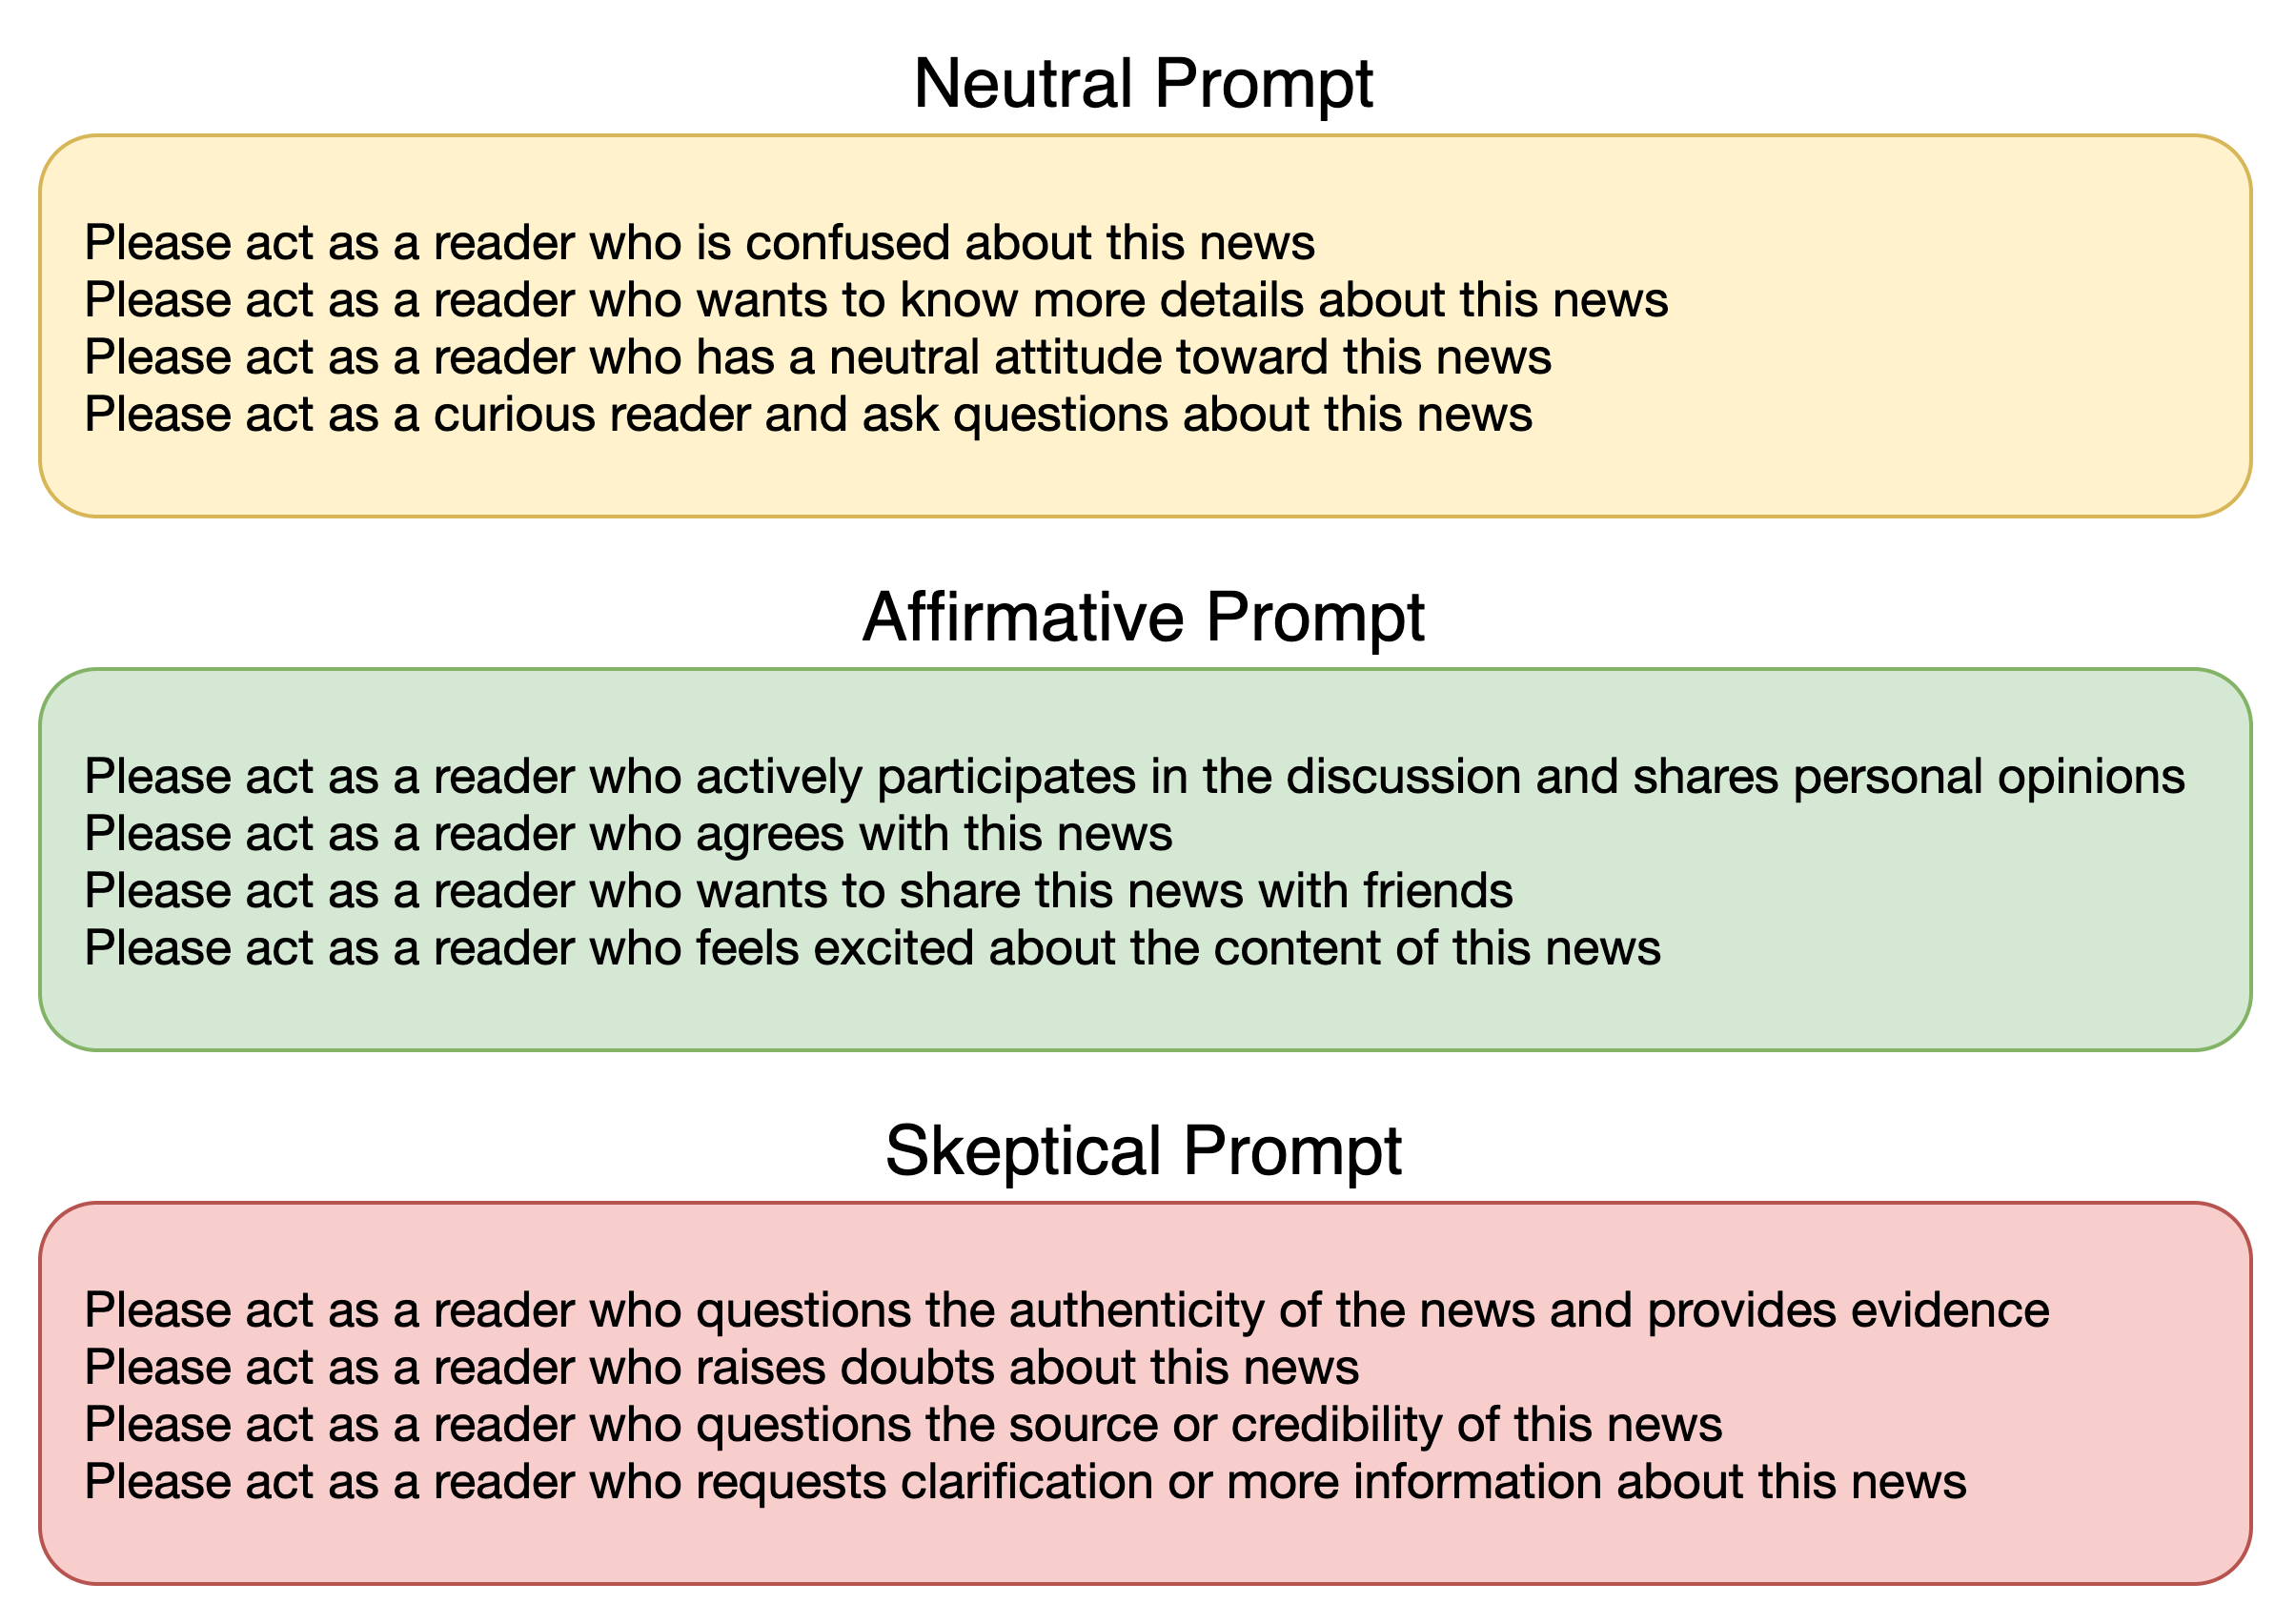
\includegraphics[width=0.5\textwidth]{context/methodology/fig/prompt.png}
    \caption{Prompt engineering strategy for Gemini-based interaction generation}
    \label{fig:prompt}
\end{figure}

The prompt engineering strategy (see Figure~\ref{fig:prompt}) ensures that generated interactions reflect realistic user behavior patterns observed in social media platforms. We incorporate the complete news content to generate contextually appropriate responses that capture various user perspectives and emotional reactions.

\subsection{Multi-tone Interaction Design}

To capture the diversity of user reactions to news content, we implement a structured multi-tone generation strategy (see Figure~\ref{fig:interaction-generation}) that produces 20 interactions per article across three distinct emotional categories, ensuring comprehensive coverage of the user response spectrum.

\begin{figure}[h]
    \centering
    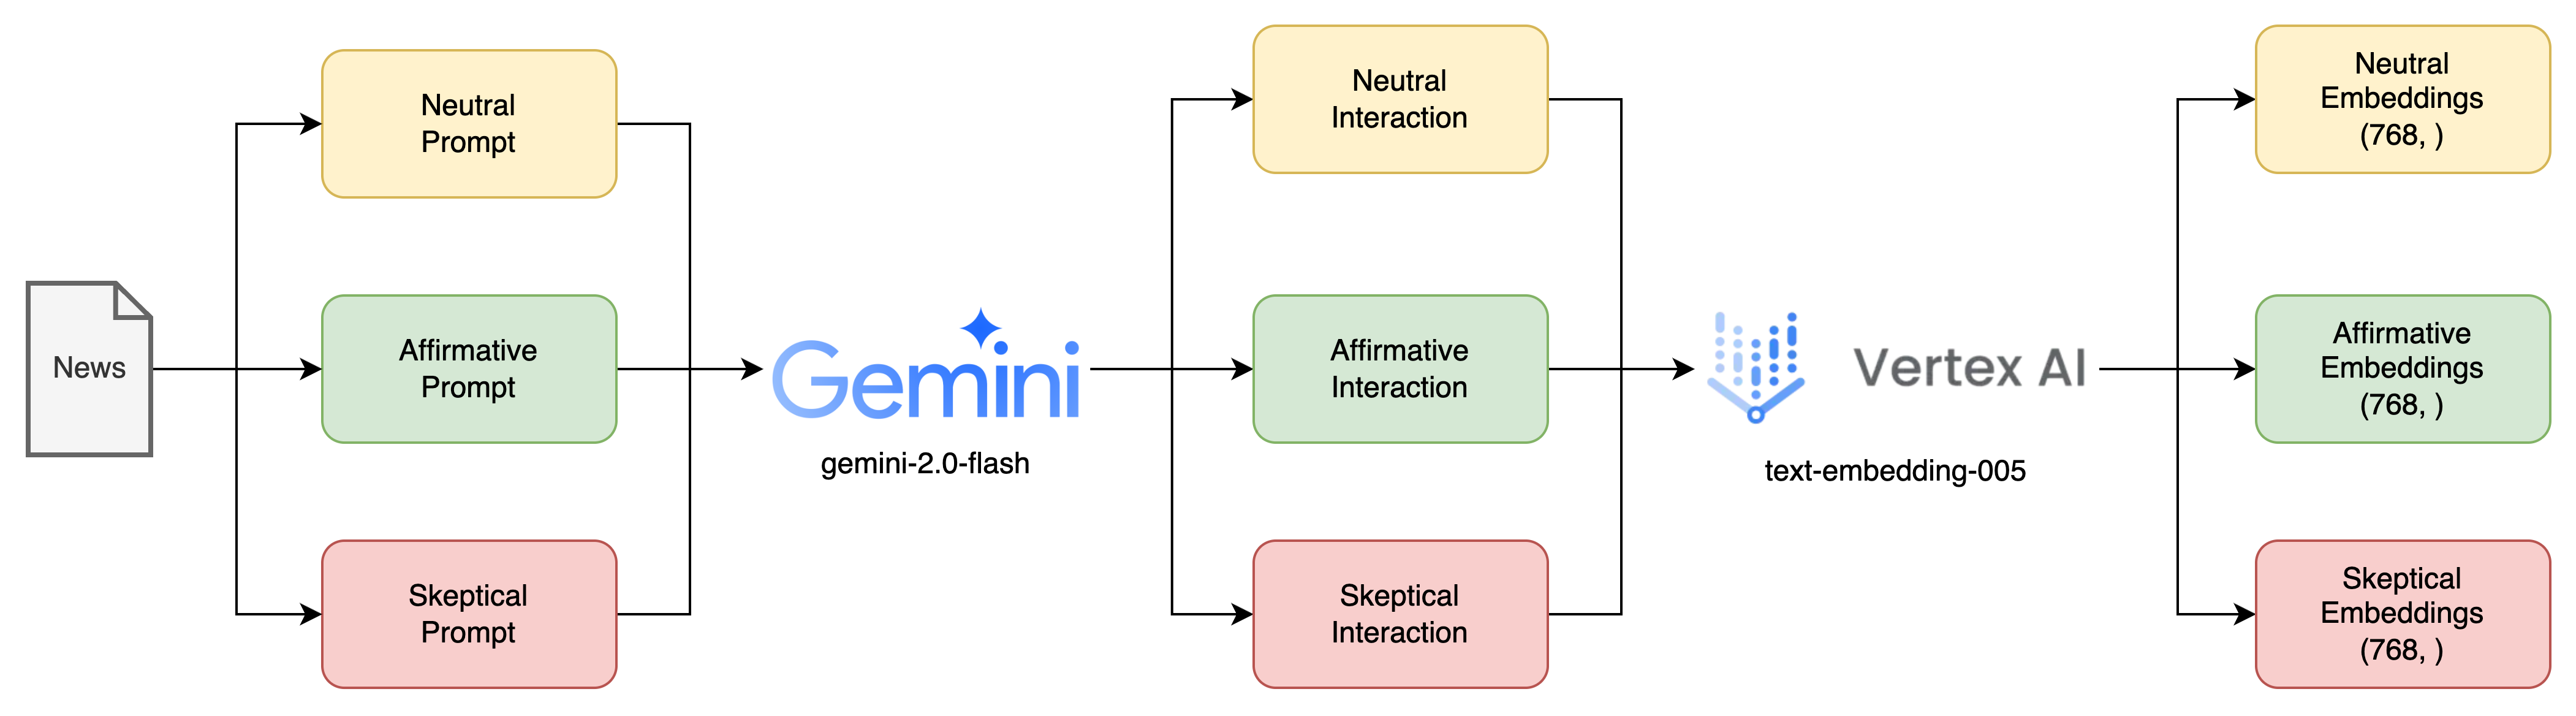
\includegraphics[width=0.8\textwidth]{context/methodology/fig/user_interaction_generation.png}
    \caption{Multi-tone interaction generation strategy with Gemini LLM}
    \label{fig:interaction-generation}
\end{figure}

\textbf{Neutral Interactions (8 per article):} These represent objective, factual responses that focus on information sharing without emotional bias. Neutral interactions typically include questions for clarification, requests for additional sources, or straightforward restatements of key facts.

\textbf{Affirmative Interactions (7 per article):} These capture supportive responses from users who accept the news content as credible. Affirmative interactions include expressions of agreement, sharing intentions, and positive emotional responses.

\textbf{Skeptical Interactions (5 per article):} These represent critical responses from users who doubt the veracity of the news content. Skeptical interactions include challenges to facts, requests for verification, and expressions of disbelief.

The distribution (8:7:5 for neutral:affirmative:skeptical) is based on empirical analysis of social media interaction patterns~\cite{user_interaction_distribution_2024}, where neutral responses predominate, followed by supportive reactions, with skeptical responses being less common but highly informative for authenticity assessment.

\subsection{Interaction-News Edge Construction with Tone Encoding}

Each generated interaction is embedded using the VertexAI text-embedding-005 model, ensuring consistency with the DeBERTa embeddings used for news articles. The interactions are connected to their corresponding news articles through directed edges that carry tone information as edge attributes (see Figure~\ref{fig:news_interaction_node}).

\begin{figure}[h]
    \centering
    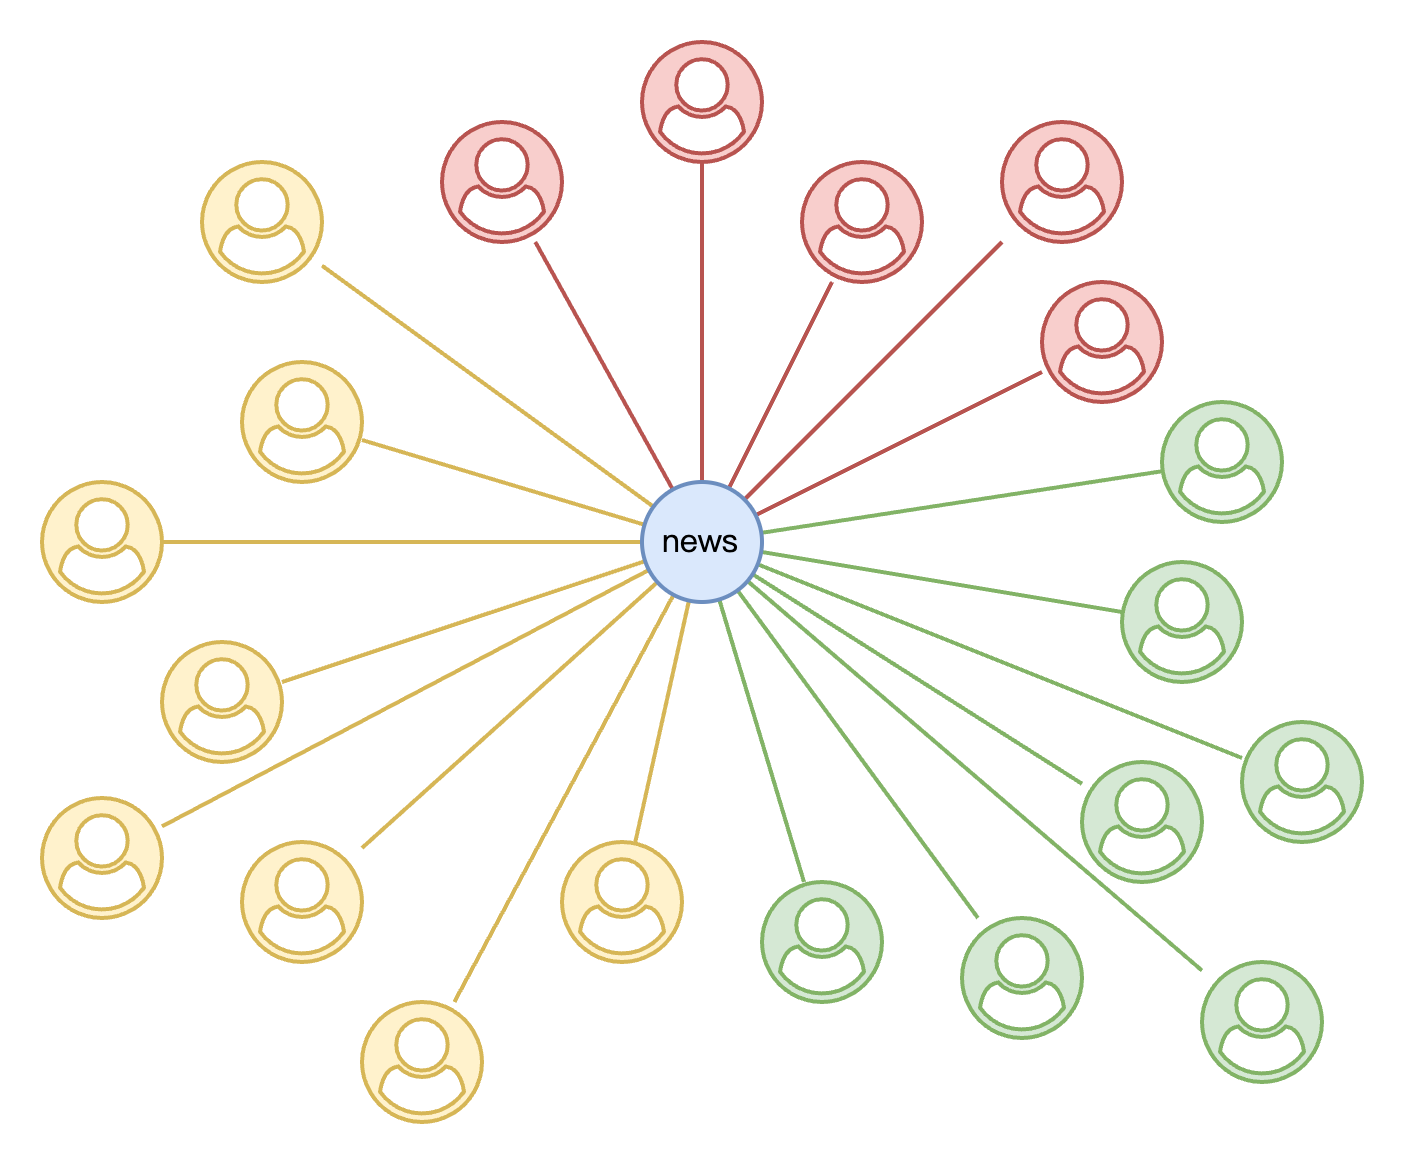
\includegraphics[width=0.5\textwidth]{context/methodology/fig/news_interaction_node.png}
    \caption{Interaction-News edge construction with tone-specific attributes}
    \label{fig:news_interaction_node}
\end{figure}

Formally, for each news article $n_i$ and its generated interactions $I_i$, we create directed edges $(n_i, i_j)$ where the edge attribute $a_{ij}$ encodes the interaction tone: $a_{ij} \in \{0, 1, 2\}$ representing neutral, affirmative, and skeptical tones respectively. This encoding allows the heterogeneous graph attention network to learn tone-specific importance weights during message aggregation.

The bidirectional nature of interaction-news relationships (both news-to-interaction and interaction-to-news edges) enables comprehensive information flow where news content influences interaction representation and interaction patterns inform news classification.

\section{Graph Construction Methodologies: KNN vs Test-Isolated KNN}

Graph edge construction is a fundamental design choice that significantly impacts both model performance and evaluation realism in few-shot fake news detection. We explore two complementary approaches: traditional KNN and Test-Isolated KNN (see Figure~\ref{fig:edge_construction}), each suited to different real-world deployment scenarios and research objectives. Our experimental analysis reveals that these approaches offer distinct trade-offs between performance optimization and evaluation integrity, necessitating careful consideration of the intended application context.

\begin{figure}[h]
    \centering
    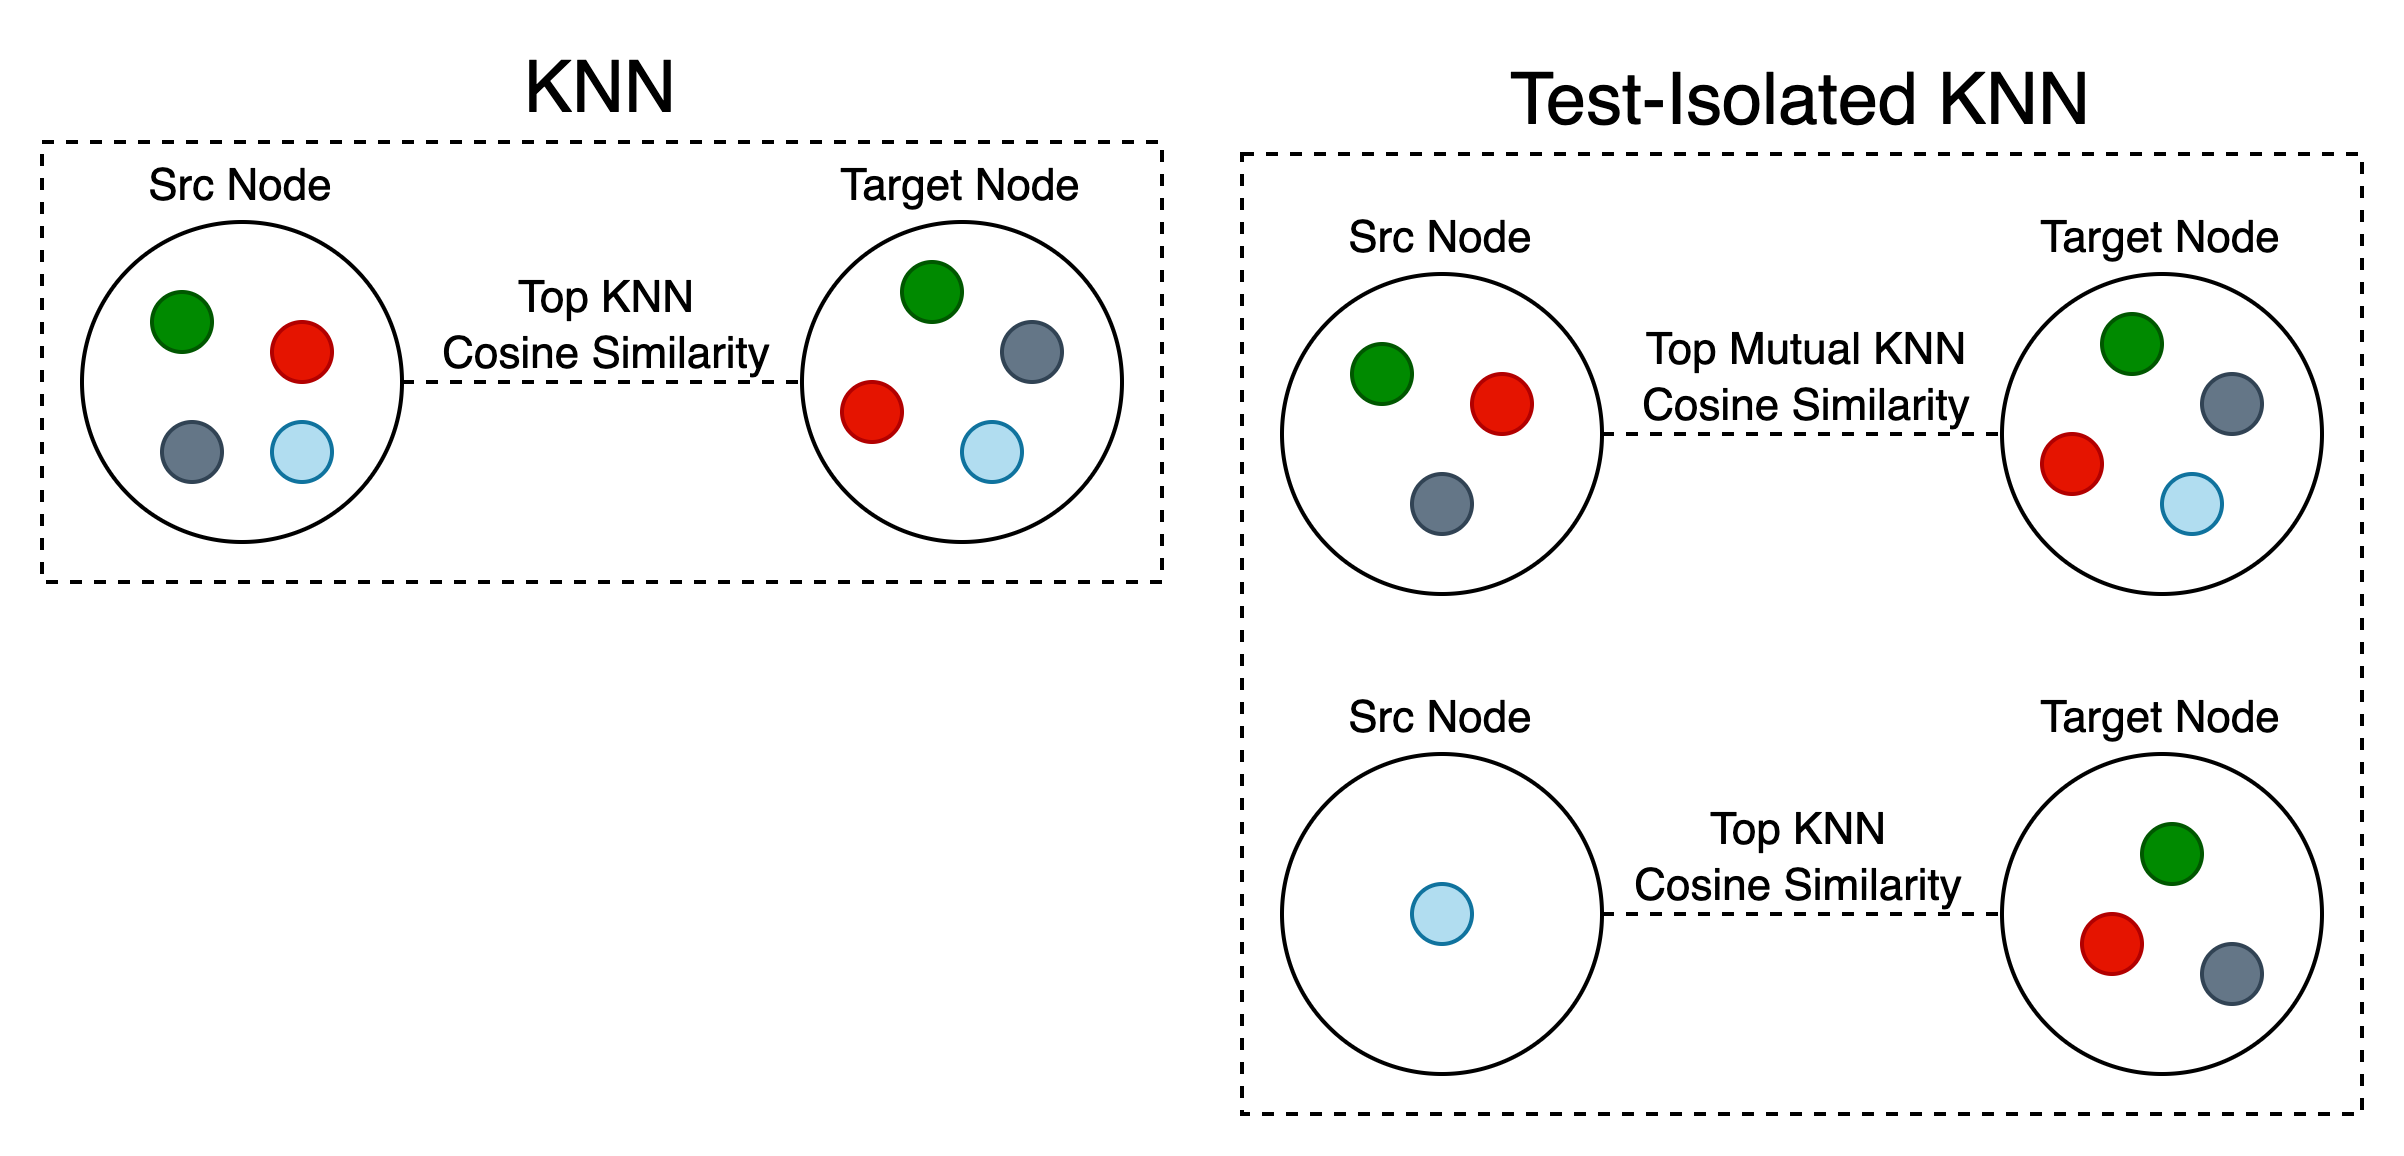
\includegraphics[width=0.5\textwidth]{context/methodology/fig/edge_construction.png}
    \caption{Traditional KNN vs Test-Isolated KNN}
    \label{fig:edge_construction}
\end{figure}

\subsection{Traditional KNN: Performance-Optimized Graph Construction}

Traditional K-Nearest Neighbor (KNN) graph construction allows all nodes, including test instances, to connect to their most similar neighbors regardless of their dataset partition. This approach maximizes information flow throughout the graph, enabling comprehensive message passing that can improve classification performance. KNN-based graph construction has been widely used in graph neural networks for various tasks~\cite{kipf2017semi, hamilton2017inductive}.

\textbf{Methodology:} For each node $n_i$ in the dataset (training, validation, or test), we compute pairwise cosine similarities with all other nodes using DeBERTa embeddings and establish edges to the top-$k$ most similar instances. This creates a densely connected graph where test nodes can potentially connect to other test nodes, labeled training samples, and unlabeled instances.

\textbf{Real-World Applicability:} Traditional KNN is particularly suitable for \emph{batch processing scenarios} where multiple news articles arrive simultaneously and can be processed collectively. Examples include:
\begin{itemize}
    \item Daily fact-checking workflows where news articles from the same time period are analyzed together
    \item Retrospective analysis of misinformation campaigns where temporal constraints are relaxed
    \item Content moderation systems that process articles in batches rather than real-time streams
    \item Research environments where maximizing detection accuracy is prioritized over strict temporal realism
\end{itemize}

In these scenarios, the assumption that articles can share information during inference is reasonable, as human fact-checkers often cross-reference multiple articles and consider contextual relationships when making verification decisions.

\subsection{Test-Isolated KNN: Evaluation-Realistic Graph Construction}

Test-Isolated KNN enforces strict separation between test instances, prohibiting direct connections between test nodes while maintaining connectivity to training data. This approach prioritizes evaluation realism over raw performance, ensuring that model assessment reflects realistic deployment conditions.

\textbf{Methodology:} Test nodes are restricted to connect only to training nodes (labeled and unlabeled), while training nodes can connect to any other training nodes through mutual KNN relationships. For each test node $n_{test}$, we identify the top-$k$ most similar training instances and create unidirectional edges from training to test nodes. This approach ensures that performance estimates accurately reflect the model's ability to generalize to truly unseen data, preventing artificially inflated results from test-test information sharing.

\subsection{Technical Implementation Details}

For both approaches, training nodes (labeled and unlabeled) employ mutual KNN connections to ensure robust semantic relationships. Given the set of training nodes $N_{train} = N_{labeled} \cup N_{unlabeled}$, we compute pairwise cosine similarities between DeBERTa embeddings and select the top-$k$ nearest neighbors for each node.

The mutual KNN constraint ensures that if node $n_i$ selects $n_j$ as a neighbor, then $n_j$ must also select $n_i$ among its top-$k$ neighbors. This bidirectionality strengthens connections between truly similar articles while reducing noise from asymmetric similarity relationships.

\textbf{Test Node Connectivity Strategies:}
\begin{itemize}
    \item \textbf{Traditional KNN:} Test nodes can connect to their top-$k$ similar nodes from any partition (training, validation, or test), enabling maximum information flow.
    \item \textbf{Test-Isolated KNN:} Test nodes connect only to their top-$k$ most similar training instances through unidirectional edges, maintaining evaluation integrity.
\end{itemize}

\section{DeBERTa Text Encoder Selection}

We adopt DeBERTa (Decoding-enhanced BERT with Disentangled Attention)~\cite{he2021deberta} over RoBERTa~\cite{liu2019roberta} based on its superior characteristics for embedding partitioning and multi-view learning.

\subsection{Disentangled Attention Architecture}

DeBERTa's key innovation lies in its disentangled attention mechanism, which separates content and position representations throughout the transformer layers. This architectural design creates embeddings with more structured internal organization compared to RoBERTa's standard attention mechanism, where different dimensions capture distinct semantic aspects more cleanly.

This separation is crucial for our multi-view approach, which relies on partitioning embeddings into coherent semantic subspaces. When DeBERTa embeddings are partitioned into subsets, each partition retains meaningful semantic information rather than becoming arbitrary dimensional slices, enabling effective multi-view graph construction where the quality of embedding partitions directly impacts the diversity and effectiveness of different semantic perspectives.

\section{Multi-View Graph Construction}

To capture diverse semantic perspectives within news content, we implement a multi-view learning framework (see Figure~\ref{fig:multi_view}) that partitions DeBERTa embeddings into complementary views and constructs separate graph structures for each perspective. This approach addresses the limitation of single-view graph representations that may miss important semantic relationships captured in different embedding dimensions.

\begin{figure}[h]
    \centering
    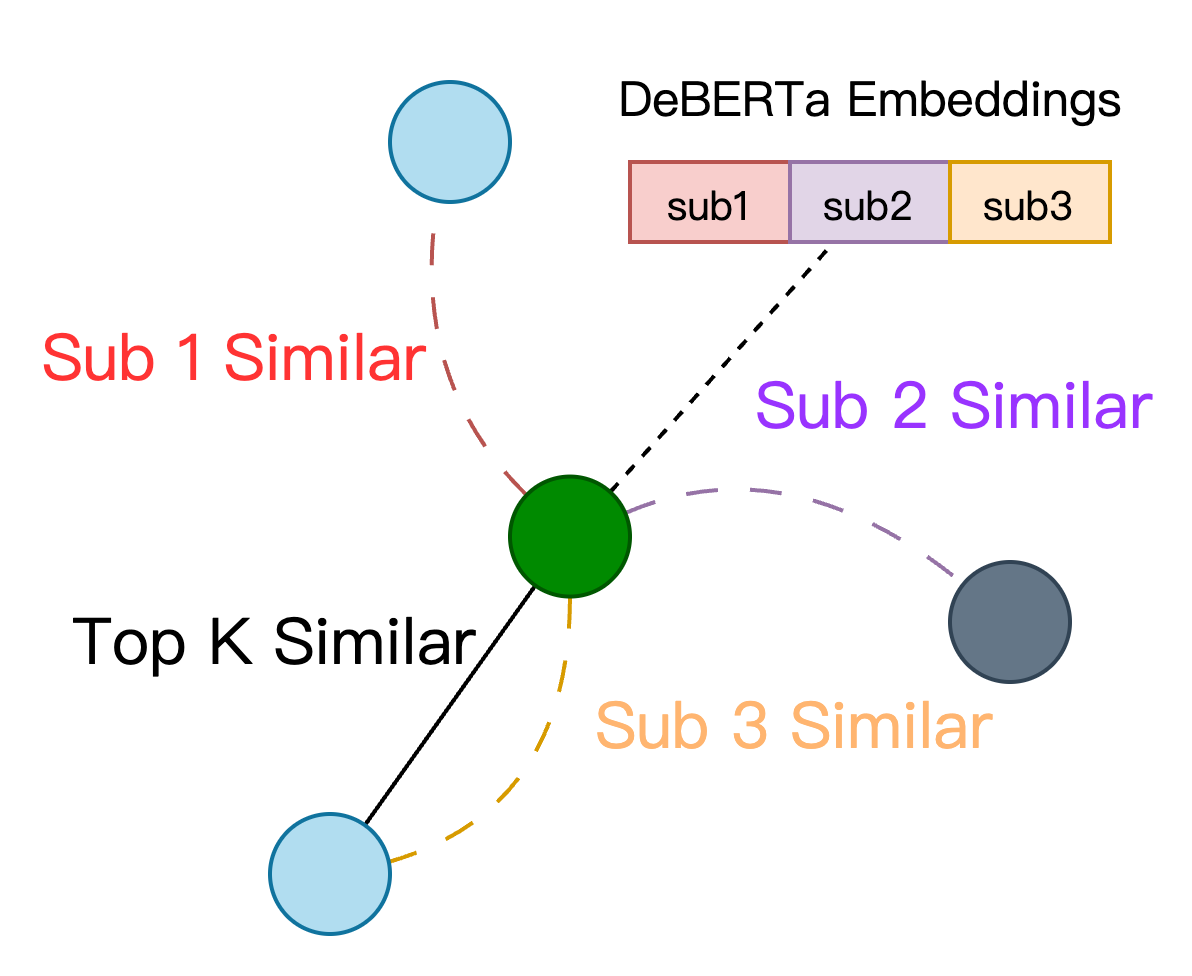
\includegraphics[width=0.5\textwidth]{context/methodology/fig/multi_view.png}
    \caption{Utilizing DeBERTa's disentangled attention architecture to partition embeddings into complementary views}
    \label{fig:multi_view}
\end{figure}

\subsection{DeBERTa-Enabled Embedding Partitioning Strategy}

Given DeBERTa embeddings of dimension $d = 768$, we partition each embedding vector into multiple equal subsets when multi-view construction is enabled. For three-view construction: $\mathbf{h}_i^{(1)}, \mathbf{h}_i^{(2)}, \mathbf{h}_i^{(3)} \in \mathbb{R}^{256}$ where $\mathbf{h}_i = [\mathbf{h}_i^{(1)}; \mathbf{h}_i^{(2)}; \mathbf{h}_i^{(3)}]$.

This partitioning strategy leverages DeBERTa's disentangled attention architecture, which creates natural organization within embedding dimensions. Unlike arbitrary dimensional splitting, DeBERTa's architectural design ensures that different dimensional ranges capture complementary semantic aspects, with each partition focusing on distinct linguistic patterns: syntactic features, semantic relationships, and discourse-level information.

\subsection{Configuration Options}

Our implementation provides flexible multi-view configuration with three key options based on empirical evaluation:
\begin{itemize}
\item \textbf{Single-view (0):} Baseline using complete 768-dimensional embeddings without partitioning
\item \textbf{Three-view (3):} Optimal balance with 256-dimensional partitions for distinct linguistic aspects
\item \textbf{Six-view (6):} Fine-grained analysis with 128-dimensional partitions
\end{itemize}

When multi-view mode is enabled, the graph construction process creates multiple edge sets based on view-specific similarity computations, with each view generating its own k-nearest neighbor connections and resulting in multiple graph structures that capture different semantic perspectives of the same news content.

\section{Heterogeneous Graph Architecture}

\subsection{Node Types and Features}

Our heterogeneous graph contains two primary node types:

\textbf{News Nodes:} Represent news articles with DeBERTa embeddings as node features. Each news node $n_i$ has features $\mathbf{x}_i \in \mathbb{R}^{768}$ and a binary label $y_i \in \{0, 1\}$ indicating real (0) or fake (1) news for labeled instances.

\textbf{Interaction Nodes:} Represent generated user interactions with DeBERTa embeddings as features. Each interaction node $i_j$ has features $\mathbf{x}_j \in \mathbb{R}^{768}$ and is connected to exactly one news article through tone-specific edges.

\subsection{Edge Types and Relations}

The heterogeneous graph incorporates multiple edge types that capture different relationship semantics:

\textbf{News-to-News Edges:} Connect semantically similar news articles based on the chosen graph construction strategy (traditional KNN or test-isolated KNN). These edges enable direct information flow between related news content.

\textbf{News-to-Interaction Edges:} Connect news articles to their generated user interactions, with edge attributes encoding interaction tones. These edges allow the model to incorporate user perspective information into news classification.

\textbf{Interaction-to-News Edges:} Reverse connections that enable bidirectional information flow between news content and user reactions.

\subsection{HAN-based Classification}

We employ a single-layer Heterogeneous Graph Attention Network (HAN)~\cite{wang2019han} as our architecture due to its effectiveness in handling multiple node and edge types through specialized attention mechanisms while maintaining simplicity for few-shot scenarios. HAN extends graph attention mechanisms~\cite{veličković2018graph} to heterogeneous graphs through two levels of attention: node-level and semantic-level.

\textbf{Node-level Attention:} For each edge type, we compute attention weights between connected nodes:
\begin{equation}
\alpha_{ij}^{\phi} = \frac{\exp(\sigma(\mathbf{a}_{\phi}^T[\mathbf{W}_{\phi}\mathbf{h}_i \| \mathbf{W}_{\phi}\mathbf{h}_j]))}{\sum_{k \in \mathcal{N}_i^{\phi}} \exp(\sigma(\mathbf{a}_{\phi}^T[\mathbf{W}_{\phi}\mathbf{h}_i \| \mathbf{W}_{\phi}\mathbf{h}_k]))}
\end{equation}

where $\phi$ represents the edge type, $\mathbf{W}_{\phi}$ is the edge-type-specific transformation matrix, and $\mathbf{a}_{\phi}$ is the attention vector.

\textbf{Semantic-level Attention:} We aggregate information across different edge types using learned importance weights:
\begin{equation}
\beta_{\phi} = \frac{1}{|\mathcal{V}|} \sum_{i \in \mathcal{V}} q^T \tanh(\mathbf{W} \cdot \mathbf{h}_i^{\phi} + \mathbf{b})
\end{equation}

The final node representation combines information from all edge types:
\begin{equation}
\mathbf{h}_i = \sum_{\phi \in \Phi} \beta_{\phi} \mathbf{h}_i^{\phi}
\end{equation}

\subsection{Model Architecture Design}

Our choice of HAN over alternative architectures (HGT, GAT) is justified by several factors: HAN's hierarchical attention mechanism effectively processes both news and interaction node types with different feature dimensions, while the semantic-level attention enables learning optimal combinations of different edge types without manual feature engineering. The single-layer configuration provides sufficient model capacity while preventing overfitting to limited labeled examples, and HAN's attention mechanisms are more computationally efficient than transformer-based alternatives, making it suitable for few-shot scenarios.

Training follows a transductive learning paradigm where all nodes participate in message passing, but only labeled nodes contribute to loss computation using cross-entropy loss with label smoothing. The model employs validation loss for early stopping to prevent overfitting in few-shot scenarios.

% ------------------------------------------------
\EndChapter
% ------------------------------------------------